\documentclass{article}
\usepackage{ismir,amsmath,cite}
\usepackage{graphicx}
\usepackage{color}
\usepackage{subcaption}

\title{Extracting Ground-Truth Information from MIDI Files}

%\oneauthor
% {Colin Raffel and Daniel P. W. Ellis}
% {LabROSA \\ Department of Electrical Engineering \\ Columbia University \\ New York, NY}

\threeauthors
  {First Author} {Affiliation1 \\ {\tt author1@ismir.edu}}
  {Second Author} {\bf Retain these fake authors in\\\bf submission to preserve the formatting}
  {Third Author} {Affiliation3 \\ {\tt author3@ismir.edu}}

%% To make customize author list in Creative Common license, uncomment and customize the next line
%  \def\authorname{Colin Raffel, Daniel P. W. Ellis} 

\sloppy

\begin{document}

\maketitle

\begin{abstract}
MIDI files abound and provide a bounty of information for music informatics.
We enumerate the types of information available in MIDI files and describe the steps necessary for utilizing them.
We also quantify the reliability of this data by comparing it to human-annotated ground truth.
The results suggest that further research in audio-to-MIDI alignment will facilitate the use of MIDI-derived ground-truth information for audio content-based MIR.
\end{abstract}

\section{MIDI Files}\label{sec:introduction}

MIDI (Music Instrument Digital Interface) is a hardware and software standard for communicating musical events.
First proposed in 1983 \cite{international1983midi}, MIDI remains a highly pervasive standard both for storing musical scores and communicating information between digital music devices.
Its use is perhaps in spite of its crudeness, which has been lamented since MIDI's early days \cite{moore1988dysfunctions}; most control values are quantized as 7-bit integers and information is transmitted at the relatively slow (by today's standards) 31,250 bits per second.
Nevertheless, its efficiency and well-designed specification make it a convenient way of formatting digital music information.

In the present work, we will focus on MIDI files, which in a simplistic view can be considered a compact way of storing a musical score.
MIDI files are specified by an extension to the MIDI standard \cite{international1988standard} and consist of a sequence of MIDI messages organized in a specific format.
A typical MIDI file contains timing and meter information in addition of a collection of one or more ``tracks'', each of which contains a sequence of notes and control messages.
The General MIDI standard further specifies a collection of 128 instrument types on which the notes can be played, which standardizes the playback of MIDI files and has therefore been widely adopted.

When paired with a General MIDI synthesizer, MIDI files have been used as a sort of (highly lossy) perceptual audio codec, with entire songs only requiring a few kilobytes of storage.
The early availability of this ``coding method'', combined with the expense of digital storage in the 90s, made MIDI files a highly pervasive method of storing and playing back songs before the advent of the MP3.
Even after high-quality perceptual audio codecs were developed and storage prices plummeted, MIDI files remained in use in resource-scarce settings such as karaoke machines and cell phone ringtones.
As a result, there is an abundance of MIDI file transcriptions of music available today; through a large-scale web scrape, we obtained 176,141 MIDI files with unique MD5 checksums.

Given their wide availability, we believe that MIDI files are underutilized in the Music Information Retrieval community.
In this paper, we start by outlining the various sources of information present in MIDI files and reference relevant works which utilize them in Section \ref{sec:information}.
In Section \ref{sec:utilizing}, we discuss the steps needed to leverage MIDI-derived information as ground truth for content-based MIR.
Based on these steps, we establish a baseline for the reliability of MIDI-derived ground truth by comparing it to handmade annotations in Section \ref{sec:measuring}.
Finally, in Section \ref{sec:discussion}, we argue that improving the process of extracting information from MIDI files is a viable path for creating large amounts of ground truth data for MIR.

\section{Information Available in MIDI Files}
\label{sec:information}

While various aspects of MIDI files have been used in MIR research, to our knowledge there has been no unified overview of the information they provide, nor a discussion of the availability and reliability of this information in MIDI transcriptions found ``in the wild''.
We therefore present an enumeration of the different information sources in a typical MIDI file and discuss their applicability to different MIR tasks.
Because not all MIDI files are created equal, we also computed statistics about the presence and quantity of each information source across our collection of 176,141 unique MIDI files; the results can be seen in Figure \ref{fig:statistics} and will be discussed in the following sections.

\begin{figure*}
    \centering
    \begin{subfigure}{.23\textwidth}
        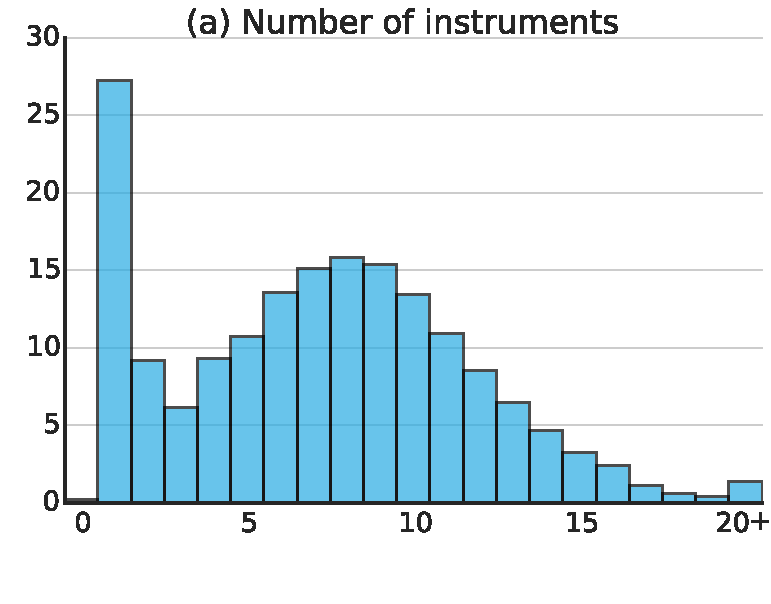
\includegraphics[width=\textwidth]{n_instruments.pdf}
    \end{subfigure}
    \begin{subfigure}{.23\textwidth}
        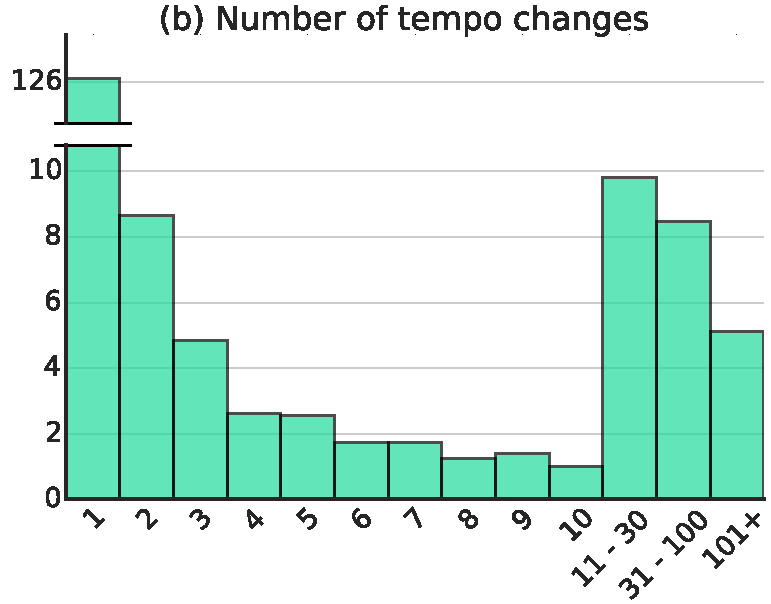
\includegraphics[width=\textwidth]{n_tempos.pdf}
    \end{subfigure}
    \begin{subfigure}{.23\textwidth}
        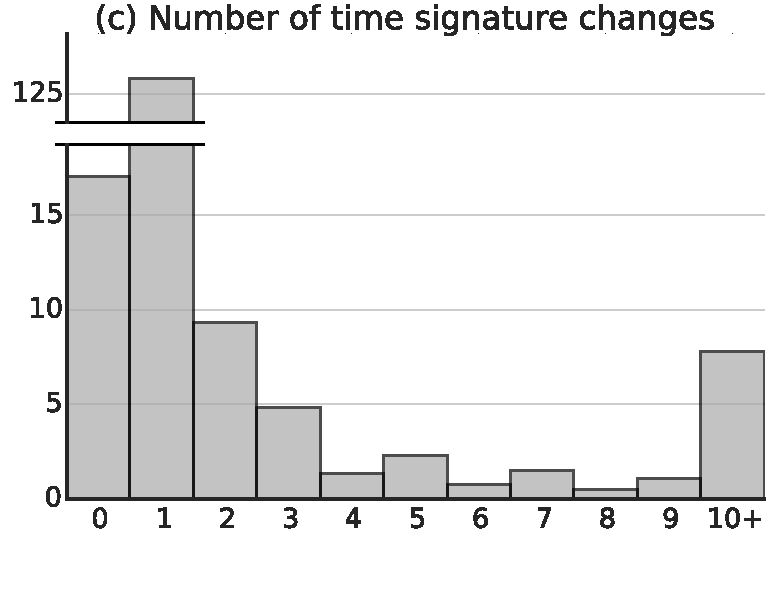
\includegraphics[width=\textwidth]{n_signatures.pdf}
    \end{subfigure}
    \begin{subfigure}{.23\textwidth}
        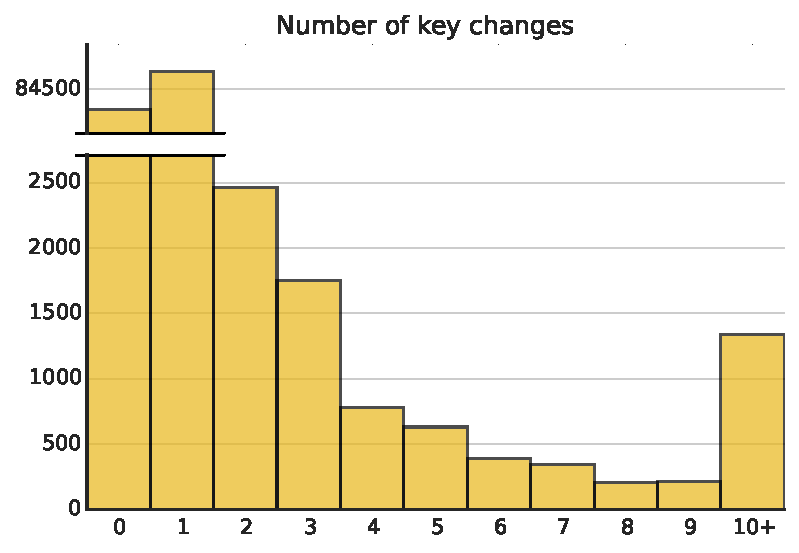
\includegraphics[width=\textwidth]{n_keys.pdf}
    \end{subfigure}

    \begin{subfigure}{.23\textwidth}
        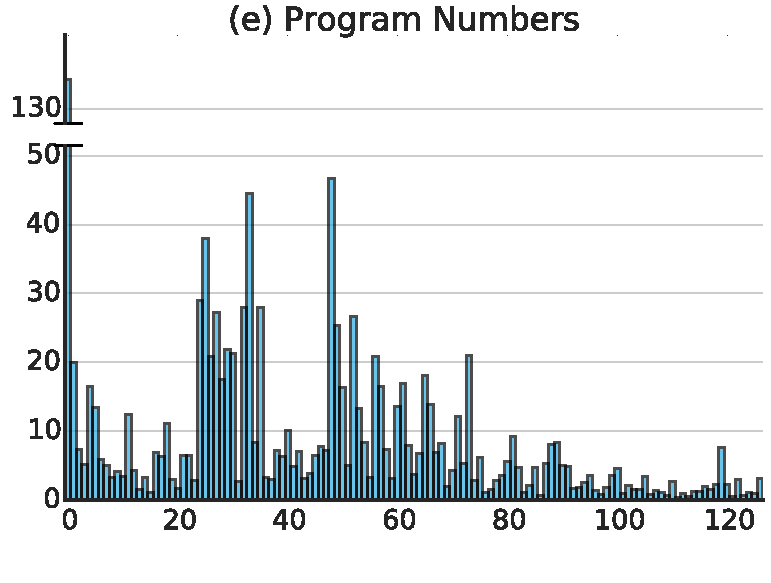
\includegraphics[width=\textwidth]{program_numbers.pdf}
    \end{subfigure}
    \begin{subfigure}{.23\textwidth}
        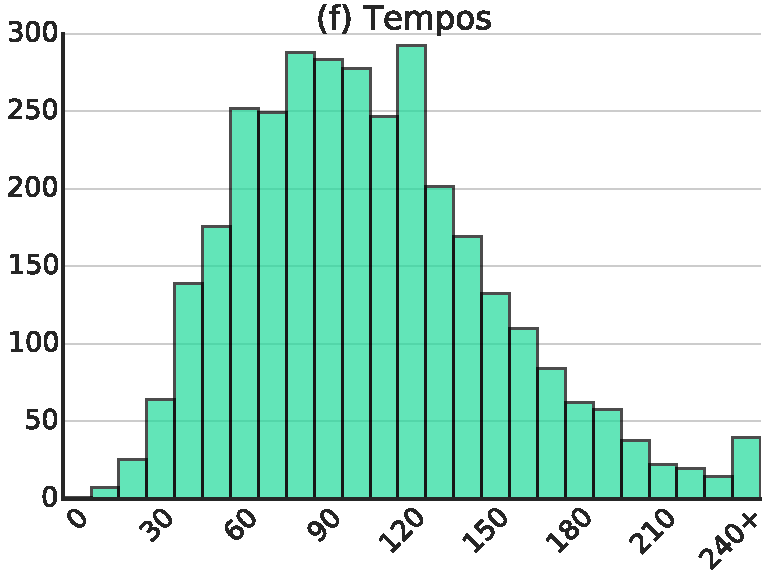
\includegraphics[width=\textwidth]{tempos.pdf}
    \end{subfigure}
    \begin{subfigure}{.23\textwidth}
        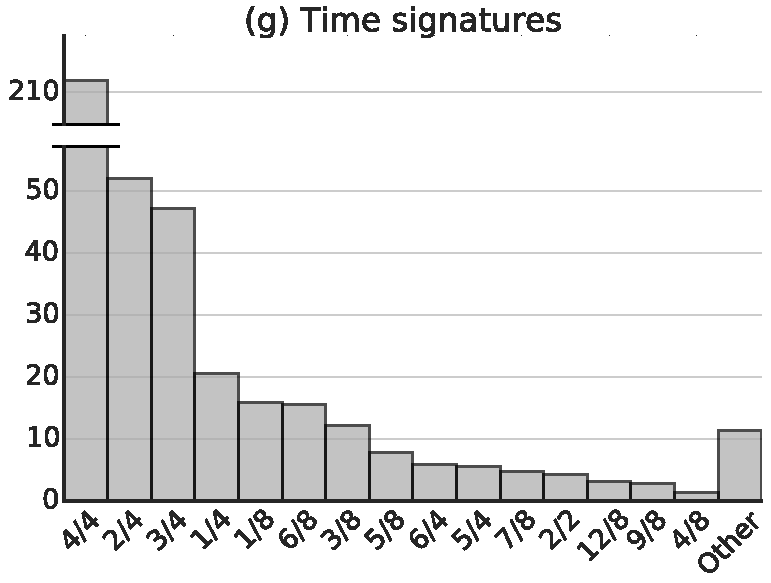
\includegraphics[width=\textwidth]{time_signatures.pdf}
    \end{subfigure}
    \begin{subfigure}{.23\textwidth}
        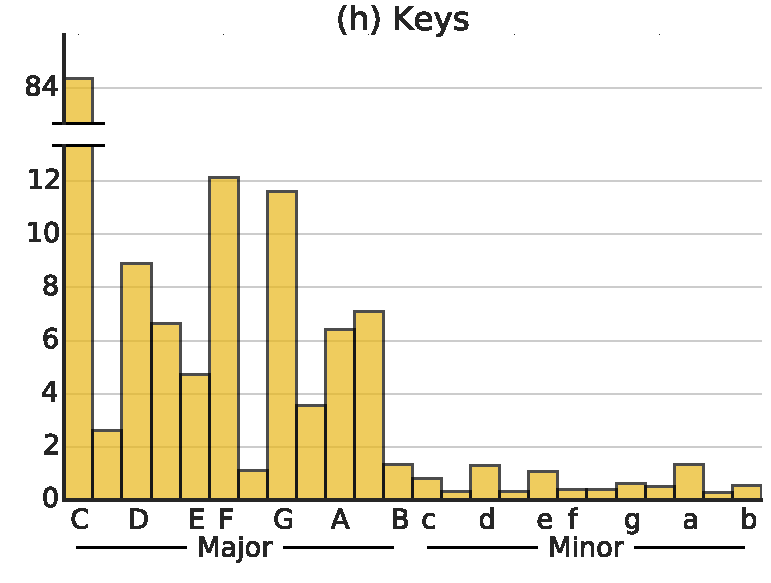
\includegraphics[width=\textwidth]{keys.pdf}
    \end{subfigure}
    \caption{Statistics about sources of information in 176,141 unique MIDI files scraped from the internet.
    Histograms in the top row show the number of MIDI files which had a given number of events for different event types; in the bottom row, we show distributions of the different values set by these events across all MIDI files.
    For example, about 125,000 MIDI files had a single time signature change event, and about 210,000 of our MIDI files included at least one 4/4 time signature.}
    \label{fig:statistics}
\end{figure*}

\subsection{Transcription}

MIDI files are specified as a collection of ``tracks'', where each track consists of a sequence of MIDI events on one of 16 channels.
Commonly used MIDI events are note on and note off messages, which together specify the start and end time of notes played at a given pitch on a given channel.
Various control events also exist, such as pitch bends, which allow for finer control of the playback of the MIDI file.
Program change events determine which instrument these events are sent to.
The General MIDI standard defines a correspondence between program numbers and a pre-defined list of 128 instruments.
The distribution of the total number of program change events (corresponding to the number of instruments) across the MIDI files in our collection and the distribution of these program numbers are shown in Figures \ref{fig:statistics}(a) and \ref{fig:statistics}(e) respectively.

This specification makes MIDI files naturally suited to be used as transcriptions of pieces of music, due to the fact that they can be considered a sequence of notes played on a collection of instruments.
As a result, many MIDI files are transcriptions and are thus commonly used as training data for automatic transcription systems (see \cite{turetsky2003ground} for an early example).
This type of data also benefits score-informed source separation methods, which utilize the score as a prior to improve source separation quality \cite{ewert2014score}.
An additional natural use of this information is for ``instrument activity detection'', i.e. determining when certain instruments are being played over the course of a piece of music.
Finally, the enumeration of note start times lends itself naturally to onset detection, and MIDI data has therefore been used for this task \cite{bello2005tutorial}.

\subsection{Musicological Features}

Because many MIDI files are transcriptions of music, they can also be used to compute high-level musicological characteristics of a given piece.
Towards this end, the software library \texttt{jSymbolic} \cite{mckay2006jsymbolic} includes functionality to extract a wide variety of features, including instrumentation, rhythm, and pitch statistics.
Similarly, \texttt{music21} \cite{cuthbert2010music21} provides a general-purpose framework for analyzing collections of digital scores (including MIDI files).
Computing these features on a collection of MIDI transcriptions is valuable for omputational musicology and can enable data-driven corpus studies.
For example, \cite{cuthbert2011feature} discusses the use of \texttt{music21} and \texttt{jSymbolic} to extract features from scores and use them to distinguish music from different composers and musical traditions.

\subsection{Meter}

Timing in MIDI files is determined by two factors: The MIDI file's specified ``resolution'' and tempo change events.
Each event within the MIDI file specifies the number of ``ticks'' between it and the preceding event.
The resolution, which is stored in the MIDI file's header, sets the number of ticks which correspond to a single beat.
The amount of time spanned by each tick is then determined according to the current tempo, as set by tempo change events.
For example, if a MIDI file has a resolution of 220 ticks per quarter note and the current tempo is 120 beats per minute,\footnote{Actually, tempo change events specify the number of microseconds per quarter beat, but this can be readily converted to beats per minute.} each tick would correspond to $60/(120*220) = 0.002\overline{27}$ seconds.
If a MIDI note-on event in this file is specified to occur 330 ticks after the previous event, then it would occur $330*0.002\overline{27} = .75$ seconds later.

The timing in a MIDI file can vary over time by including many tempo change events.
In practice, as shown in Figure \ref{fig:statistics}(b), most MIDI files only contain a single tempo change and are therefore transcribed at a fixed tempo.
However, there are many MIDI files in our collection which have a large number of tempo change events (as indicated by the rightmost bars in Figure \ref{fig:statistics}(b)).
We have found that this is a common practice for making the timing of a MIDI transcription closely match that of an audio recording of the same song.
Despite the fact that the default tempo for a MIDI file is 120 beats per minute, Figure \ref{fig:statistics}(c) demonstrates that a wide range of tempos are used.
In practice, we find that this is due to the fact that even when a single tempo event is used, it is often set so that the MIDI transcription's approximates that of an audio recording of the same song.

Time signature change events further augment MIDI files with the ability to specify time signatures, and are also used to indicate the start of a measure.
By convention, MIDI files have a time signature change at the first tick, although this is not a requirement.
Because time signature changes are relatively rare in western popular music, the vast majority of the MIDI files in our collection contain a single time signature change, as seen in Figure \ref{fig:statistics}(c).
Despite the fact that 4/4 is the default time signature for MIDI files and is pervasive in western popular music, a substantial portion (about half) included a non-4/4 time signature, as shown in Figure \ref{fig:statistics}(g).

Because MIDI files are required to include tempo information in order to specify their timing, it is straightforward to extract beat locations from a MIDI file.
By convention, the first (down)beat in a MIDI transcription occurs at the first tick.
Determining the beat locations in a MIDI file therefore involves computing beat locations starting from the first tick and adjusting the tempo and time signature according to any tempo change or time signature change events found.
Despite this capability, to our knowledge MIDI files have not been used as ground-truth for beat tracking algorithms.
However, \cite{mauch2012corpus} utilized a large dataset of MIDI files to studydrum patterns using natural language processing techniques.


\subsection{Key}

An additional useful event in MIDI files is the key change event.
Any of the 24 major or minor keys may be specified.
Key changes simply give a suggestion as to the tonal content and do not effect playback, and so are a completely optional meta-event.
As seen in Figure \ref{fig:statistics}(d), this results in many MIDI files omitting key change events altogether.
A further complication is that a disproportionate number (about half) of the MIDI files in our collection had key changes to the key of C major.
This disagrees with corpus studies of popular music, e.g. \cite{carlton2012analyzed} which found that only about 26\% of songs from the Billboard 100 were in C major.
We believe this is because many MIDI transcription software packaged automatically insert a C major key change at the beginning of the file.

\subsection{Lyrics}

Lyrics can be added to MIDI transcriptions by the use of lyrics meta-events, which allow for timestamped text to be included over the course of the song.
This capability enables the common use of MIDI files for karaoke; in fact, a separate file extension ``.kar'' is often used for MIDI files which include lyrics meta-events.
Occasionally, the generic text meta-event is also used for lyrics, but this is not its intended use.
In our collection, we found about 23,801 MIDI files which had at least one lyrics meta-event (about 13.3\%).

\subsection{What's Missing}
\label{sec:missing}

Despite the wide variety of information sources available in MIDI files outlined in the previous sections, there are various types of information for which it is not possible (or not common) to store in MIDI files.
While the General MIDI specfication provides a mapping between program numbers and instrument types, none of these instruments are ``voice'' instruments except for programs 52, 53, 54, 85, and 91, which correspond to ``Choir Aahs'', ``Voice Oohs'', ``Synth Choir'', ``Lead 6 (voice)'' and ``Pad 4 (choir)'' respectively.
In practice, there is no specific program number (or numbers) which is consistently used to transcribe vocals.
As a result, in a given MIDI file there is no reliable way of determining which voice or instrument is a transcription of the vocals in a song.
Furthermore, because many MIDI files were designed for karaoke, the vocals may not be transcribed at all.

While the MIDI specification does include a ``track name'' meta-event, it is seldom used and there is no standard for its use, and so MIDI files are further constrained to the general MIDI specification.
It follows that there is no simple way to retrieve the ``melody'' from a MIDI transcription, although the fact that all instruments are transcribed separately can make its estimation more straightforward than for audio files.
To our knowledge, there has been no research into automatically determining which instrument in a given MIDI file is a transcription of the melody or vocal line.

There is also no explicit way for MIDI files to include chord labels or structural segmentation boundaries (e.g. ``verse'', ``chorus'', ``solo'').
While this would in principle be possible thanks to the generic MIDI ``text'' meta-event, we have yet to find any MIDI files which store this information.
Nevertheless, estimating chords in particular is greatly facilitated by the presence of a ground-truth transcription.
Both \texttt{music21} \cite{cuthbert2010music21} and \texttt{melisma} \cite{sleator2001melisma} include functionality for estimating chord sequences from symbolic data.

While text meta-events could also be used to store song-level metadata (song title, artist name, etc.) in a MIDI file, we have seldom encountered this in practice.
As a result, there is no standardized way to store this metadata in a MIDI file, although we found that a small portion of the filenames in our collection indicated the song title and occasionally the artist name.
The lack of a metadata specification also prevents MIDI transcriptions from being attributed to the person who transcribed them.

\section{Utilizing MIDI Files as Ground Truth}
\label{sec:utilizing}

Utilizing MIDI files as ground-truth information for audio-content based MIR tasks requires the following:
First, the artist and song of a MIDI file must be determined and it must be matched to an audio recording of the song it is a transcription of.
Second, for many information sources, the MIDI file must be aligned in time with its matching audio recording.
Finally, the compact low-level binary format used by MIDI files must be parsed so that the information can be readily extracted.

\subsection{Matching}

Apart from metadata-agnostic corpus studies such as the one in \cite{mauch2012corpus}, determining what song a given MIDI file is is often a requirement.
Matching a given MIDI file to, for example, a corresponding entry in the Million Song Dataset \cite{bertin2011million} can be beneficial even in experiments solely involving symbolic data analysis because it can provide additional useful information about the MIDI file such as the song's year, genre, and user-applied tags.
Utilizing information in a MIDI file for ground-truth in audio content-based MIR tasks further requires that it be matched to an audio recording of the song.
Unfortunately, the lack of a standardized method for storing song-level metadata in MIDI files (as discussed in Section \ref{sec:missing}) complicates this necessity.
This has prompted the development of content-based matching methods; for example, early work by \cite{hu2003polyphonic} utilized the dynamic time warping (DTW) distance to compare spectrograms of MIDI syntheses and audio files and assigned matches by finding the minimal distance within the corpus.
This approach is prohibitively slow for very large collections of MIDI and/or audio files, so \cite{raffel2015large} explored learning a mapping from spectrograms to downsampled sequences of binary vectors, which greatly accelerates DTW.
\cite{raffel2016pruning} provided further speed-up by mapping entire spectrograms to fixed-length vectors in a Euclidean space where similar songs are mapped close together.
These methods make it feasible to quickly match a MIDI file to an extremely large corpus of audio recordings.

\subsection{Aligning}

There is no guarantee that a MIDI trancsription for a given song was transcribed so that its timing matches an audio recording of a performance of the song.
For the many sources of ground-truth data which depend on timing (e.g.\ beats, transcrtiption, or lyrics), the MIDI file must therefore have its timing adjusted so that it matches that of the performance.
Fortunately, there has been a great deal of research into score-to-audio alignment, and MIDI-to-audio alignment can be seen as a special ``offline'' case.
A highly common method is to use DTW or another edit-distance measure to find the best alignment between spectrograms of the synthesized MIDI and audio recording; see \cite{raffel2016optimizing} for a survey.

In practice, audio-to-MIDI alignment systems can fail when there are overwhelming differences in timing or issues in the transcription, e.g. missing or incorrect instrumentation and/or notes.
Ideally, the alignment and matching processes could automatically report the success of the alignment and the quality of the MIDI transcription.
\cite{raffel2016optimizing} explores the ability of DTW-based alignment systems to automatically report a ``confidence'' score which denotes whether the alignment was successful or not.
To our knowledge, there has not been any research into automatically determining the quality of a MIDI transcription.

\subsection{Extracting Information}

The information sources enumerated in Section \ref{sec:information} are not readily available from MIDI files due to fact that they follow a low-level binary protocol.
For example, in order to extract the time (in seconds) of all onsets from a given instrument in a MIDI file, note events which occur on the same track and channel as program change events for the instrument must be collected and their timing must be computed from their relative ticks using the global tempo change events.
Fortunately, various software libraries have been created to facilitate this process.

The python library \texttt{pretty\char`_midi} \cite{raffel2014pretty_midi} simplifies the extraction useful information from MIDI transcriptions by taking care of most of the low-level parsing needed to convert the information to a more human-friendly format.
For example, it contains functions for retrieving beats, onsets, note lists from specific instruments, and the times and values of key, tempo, and time signature changes.
It also can be used to modify MIDI files, as well as to convert them to synthesized audio or a spectrogram-like piano roll representation.
The aforementioned Java library \texttt{jSymbolic} contains an extensive collection of routines for computing musicological features from MIDI files.
Finally, both \texttt{music21} and \texttt{melisma} are capable of inferring high-level music information from symbolic data of various types, including MIDI.

\section{Measuring a Baseline of Reliability for MIDI-Derived Information}
\label{sec:measuring}

Given the potential availability of ground-truth information in MIDI transcriptions, a natural question is the reliability of this data in MIDI transcriptions found ``in the wild''.
A straightforward way to evaluate the quality of data derived from a MIDI transcription of a given song would be to compare it to pre-existing hand-made annotations for the song.
Given a MIDI transcription and human-annotated ground truth data, we can extract corresponding information from the MIDI file and compare using the heuristic evaluation metrics commonly used in the Music Information Retrieval Evaluation eXchange (MIREX) \cite{downie2008music}.
We therefore leveraged the Isophonics Beatles annotations \cite{mauch2009omras2} as a source of ground-truth to compare against MIDI-derived information because MIDI transcriptions of these songs are readily available due to The Beatles' popularity.

Our choice in tasks depends on the overlap in sources of information in the Isophonics annotations and MIDI transcriptions.
Isophonics includes beat times, song-level key information, chord changes, and structural segmentation.
As noted in Section \ref{sec:information}, beat times and key changes may be included in MIDI files but there is no way to include chord change or structural segmentation information.
We therefore performed experiments to evaluate the quality of key labels and beat times available in MIDI files.
Fortuitously, these two experiments give us an insight into both song-level timing-agnostic information (key) and alignment-dependent timing-critical information (beat).

To carry out these experiments, we first manually identified 545 MIDI files from our collection which had filenames indicating that they were transcriptions of songs from the Isophonics Beatles collection.
Of the 180 songs in the Isophonics Beatles collection, we found MIDI transcriptions for all but 11.
The median number of MIDI transcriptions per song was 2; the song ``Eleanor Rigby'' had the most, with 14 unique transcriptions.

\subsection{Key Experiment}

\subsection{Beat Experiment}

\section{Discussion}
\label{sec:discussion}

As-is, a lot of the information is usable.

Improving audio-to-MIDI alignment as a proxy for getting additional metadata.

Many additional avenues for improvement of measuring quality.

More information sources: Guitar Pro, MusicXML

\bibliography{refs}

\end{document}
